\documentclass{beamer}
\usetheme{Darmstadt}
\usecolortheme{default}

% balíčky

\usepackage[utf8]{inputenc}
\usepackage[czech]{babel}
\usepackage{graphicx}
\usepackage{mathtools}
\DeclarePairedDelimiter\ceil{\lceil}{\rceil}
\DeclarePairedDelimiter\floor{\lfloor}{\rfloor}



% informace o dokumentu

\title[krátký titulek prezentace]{Sundaramovo síto}
\subtitle[krátký název prezentace]{A srovnání se sítem Eratosthenovým}
\author{Autor: \textbf{Marco Souza de Joode}, G. Nad Štolou}

\date{\today}

% text dokumentu

\begin{document}

% titulní stránka
% (název prezentace, autor, datum...)

\begin{frame}
  \titlepage
\end{frame}

% osnova prezentace
% (většinou se pro délku vypouští)


% obsah prezentace
% (používají se klasické sekce)

\section{Teoretický úvod}


\begin{frame}

  \frametitle{Eratosthenovo síto}
  \framesubtitle{}
  % ...


\begin{itemize}

\item Předpokládáme, že všechna čísla jsou prvočísla
\item Postupně odstraňujeme všechny celočíselné násobky
\item Případně pouze celočíslené násobky čísel, které nebyly odstraněny.
\end{itemize}
	 

\end{frame}






\begin{frame}

  \frametitle{Myšlenka za Sundaramovým sítem}
  \framesubtitle{}
  % ...


Všechna přirozená čísla jsou buď sudá nebo lichá.
Všechna prvočísla, až na číslo 2, jsou lichá. \textbf{Sundaramovo síto} selektivně vybírá složená lichá čísla a odstraňuje je.	 

\end{frame}



\begin{frame}
  \frametitle{Součiny čísel podle parity}
 
Označíme-li si sudá čísla jako $S$ a lichá čísla jako $L$, pak platí
\begin{align*}
S\cdot S &= S\\
S \cdot L &= S\\
L \cdot S &= S\\
L \cdot L &= L
\end{align*}

protože
\begin{align*}
2n \cdot 2m &= 4nm = 2 \cdot 2nm\\
2n \cdot (2m+1) &= 4nm + 2n = 2 \cdot (2nm + n) \\
(2n +1) \cdot (2m+1) &= 4nm + 2n + 2m + 1 = 2 \cdot (n + m + 2nm) + 1
\end{align*}


\end{frame}




\begin{frame}
  \frametitle{Složená lichá čísla}

Všechna lichá čísla jsou buď prvočísla, nebo čísla složená. Každé liché složené číslo lze zapsat jako

\begin{align*}
&(2i + 1)(2j +1)\\
&= 4ij + 2i + 2j +1\\
&= 2(\underbrace{i + j + 2ij}_{U}) + 1
\end{align*}


\end{frame}



\begin{frame}
  \frametitle{Základní princip Sundaramova síta}

\begin{itemize}

\item Mějme $m = \floor{N/2}$
\item Pro všechna $i \in \{1, 2,..., m\}$ a pro všechna $j \in \{1, 2,..., m\}$ nalezněme množinu čísel $L$, které \textbf{nelze} zapsat jako $U = i+j+2ij$, když $U<m$.

\item Všechna lichá prvočísla lze zapsat jako $2U + 1$ pro každé $U$ v množině $L$.
\end{itemize}

\end{frame}




\begin{frame}
  \frametitle{Optimalizace Sundaramova síta}

\begin{itemize}

\item Mějme $m = \floor{N/2}$
\item Pro všechna $i \in \{1, 2,..., m\}$, aby $U = i+j+2ij < m$, musí platit omezení na $j$:

\begin{align*}
i+j+2ij &< m\\
j(2i+1) &< m-i\\
j &< \frac{m-i}{2i+1}
\end{align*}  
a zároveň nemusíme prověřovat $j \leq i$. Pak $j \in \{i, i+1,..., \frac{m-i}{2i+1}\}$

\item Všechna lichá prvočísla lze zapsat jako $2U + 1$ pro každé $U$ v množině $L$.
\end{itemize}

\end{frame}


\section{Implementace a časová složitost}
\subsection{Eratosthenes}

\begin{frame}
  \frametitle{Eratosthenovo síto}
\begin{figure}
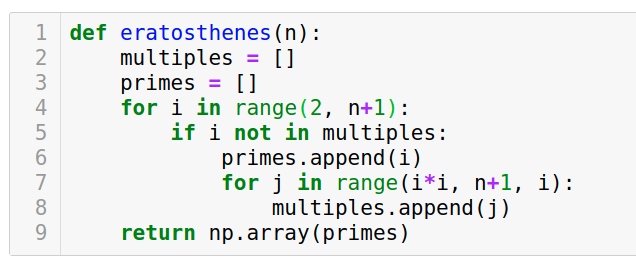
\includegraphics[height=3.5cm]{img/e1.png}
\end{figure}
Budované pomocí dvou seznamů
\begin{itemize}
\item Seznamu násobků
\item Seznamu složených čísel
\end{itemize}
\end{frame}


\begin{frame}
  \frametitle{Naivní Eratosthenovo síto pomocí Booleovských masek}
\begin{figure}
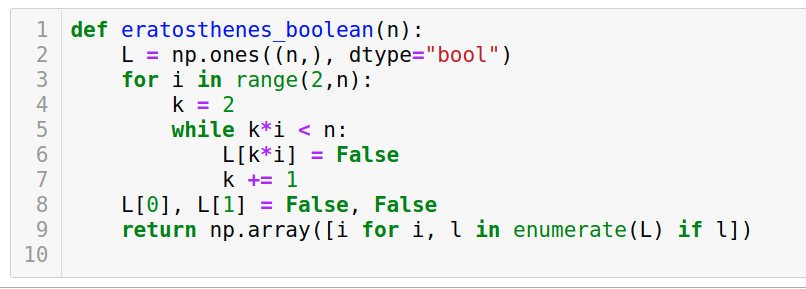
\includegraphics[height=3.5cm]{img/e2.png}
\end{figure}
Používá pouze jedno \texttt{numpy} pole zaplněné booleovskými hodnotami \texttt{True}, poté odstraňuje (naivně) všechny násobky všech čísel. 
\end{frame}


\begin{frame}
  \frametitle{Optimalizované Eratosthenovo síto}
\begin{figure}
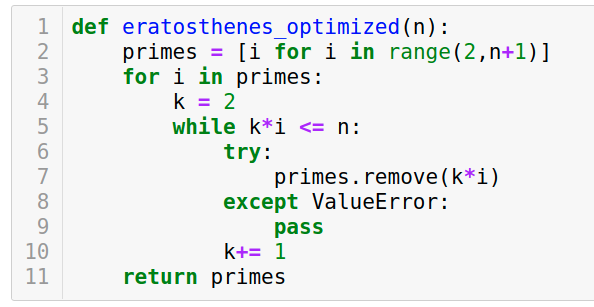
\includegraphics[height=3.5cm]{img/e3.png}
\end{figure}
Na začátku mají všechna čísla status prvočísla. Následně jsou odstraňovány všechny násobky zbývajících čísel s tímto statusem. 
\end{frame}



\begin{frame}
  \frametitle{Vzájemné srovnání}
\begin{figure}
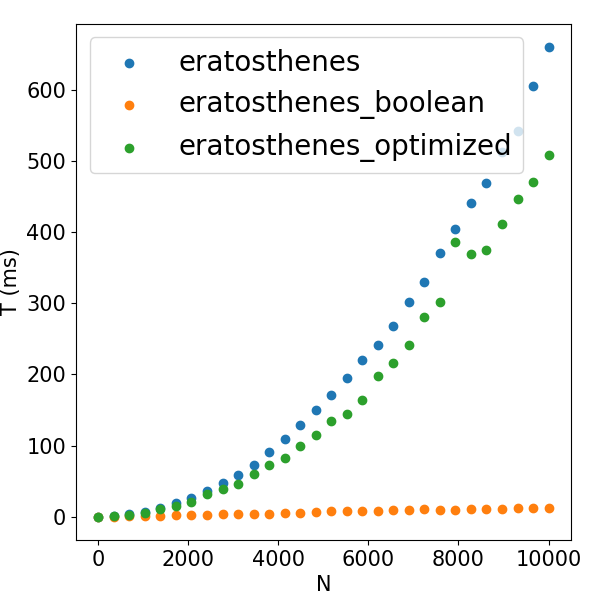
\includegraphics[height=5cm]{img/e_c.png}
\end{figure}
Vyhrává síto využívající booleovské masky. 
\end{frame}


\begin{frame}
  \frametitle{Časová složitost Eratosthenova síta}
 
Něco jako nejlepší nebo nejhorší případ zde nehraje roli - vždy procházíme tentýž seznam čísel.Za předpokladu, že odstranění složeného čísla provedeme v čase $O(1)$, tak odstranění všech násobků vyžaduje minimálně

 \begin{equation}
 O(\frac{N}{2} + \frac{N}{3} + \frac{N}{5} +  \frac{N}{7} +... + \frac{N}{p})
 \end{equation}
 
 kde $p$ je nejvyšší prvočíslo takové, že $p < N$. 
 
\end{frame}



\begin{frame}
  \frametitle{Časová složitost Eratosthenova síta}
Euler (1737) dokazuje, že
\begin{equation}
\sum_{\textrm{p je prv.}<N} \frac{1}{p} \geq \log \log (N+1) - \log \frac{\pi^2}{6}
\end{equation}
Což pro velké hodnoty $N$
 \begin{equation}
 \log \log (N+1) - \log \frac{\pi^2}{6} \approx \log \log (N)\,,
 \end{equation}
 
 a tak
 
  \begin{equation}
 O ( \frac{N}{2} + \frac{N}{3} + \frac{N}{5} +  \frac{N}{7} +... + \frac{N}{p}) \approx O(N\log \log N)\,.
 \end{equation}
\end{frame}

\subsection{Sundaramovo síto}

\begin{frame}
  \frametitle{Naivní Sundaramovo síto}
\begin{figure}
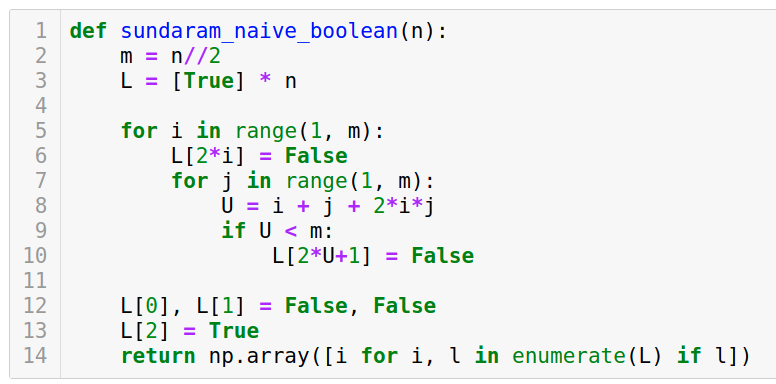
\includegraphics[height=5cm]{img/s1.png}
\end{figure}

Pomocí seznamu Booleovských hodnot. Odstraňuje čísla na indexech $U = i+j+2ij$ menší než $m = \floor{N/2}$.
\end{frame}

\begin{frame}
  \frametitle{Časová složitost naivního Sundaramova síta}
Prochází všechny body v kartézském součinu $$i \in \{2,..., \floor{N/2}\} \times j \in \{2,..., \floor{N/2}\}$$
a operuje tedy minimálně s časem

\begin{equation}
O(\floor{N/2}^2) \approx O(\frac{1}{4} N^2) \approx O(N^2) 
\end{equation}
což oproti nejlepšímu Eratosthenovu sítu představuje výrazné zhoršení.
\end{frame}

\begin{frame}
  \frametitle{Naivní Sundaramovo síto, implementace pomocí množin}
\begin{figure}
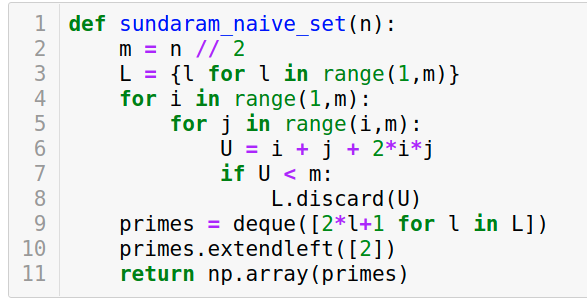
\includegraphics[height=3.5cm]{img/s2.png}
\end{figure}
Povšimneme si, že není třeba procházet celý prostor $$i \in \{2,..., \floor{N/2}\} \times j \in \{2,..., \floor{N/2}\}$$
ale stačí pouze
$$i \in \{2,..., \floor{N/2}\} \times j \in \{i,i+1,..., \floor{N/2}\}$$

\end{frame}

\begin{frame}
  \frametitle{Optimalizace Sundaramova síta}
\begin{figure}
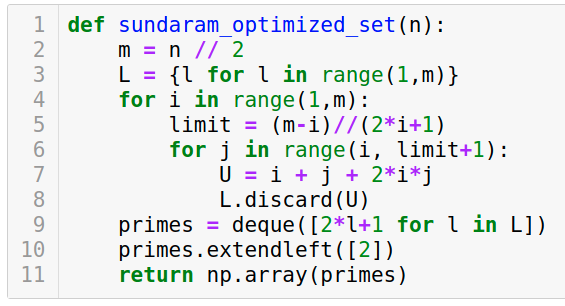
\includegraphics[height=3cm]{img/s3.png}
\end{figure}

\end{frame}


\begin{frame}
  \frametitle{Optimalizace Sundaramova síta}
Protože
\begin{align*}
i+j+2ij &< m\\
j(2i+1) &< m-i\\
j &< \frac{m-i}{2i+1}
\end{align*}  
a zároveň nemusíme prověřovat $j \leq i$. Pak $j \in \{i, i+1,..., \frac{m-i}{2i+1}\}$
\end{frame}


\begin{frame}
  \frametitle{Optimalizace Sundaramova síta pomocí Booleovské masky}
\begin{figure}
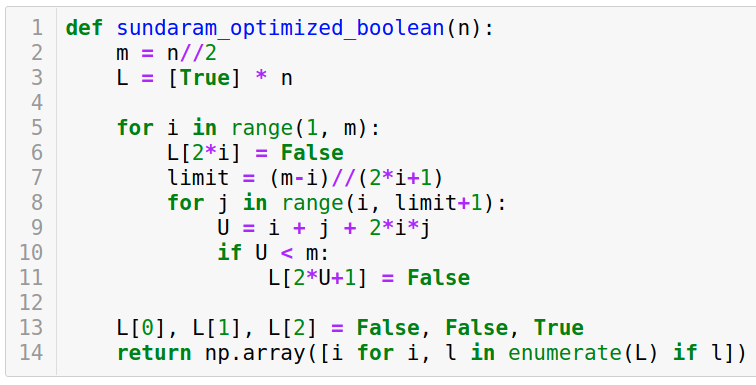
\includegraphics[height=5cm]{img/s4.png}
\end{figure}
\end{frame}


\begin{frame}
  \frametitle{Idealizovaná časová složitost}
 Časová složitost je závislá na počtu kroků, který si můžeme spočíst uměle:
\begin{figure}
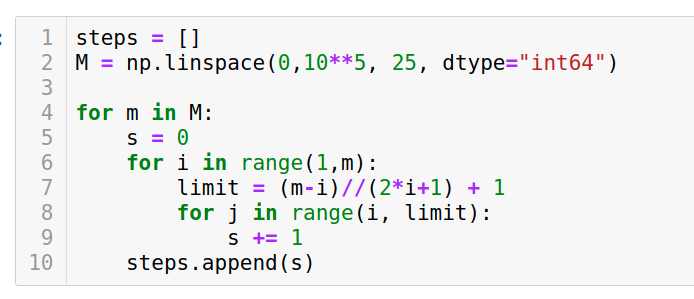
\includegraphics[height=5cm]{img/id1.png}
\end{figure}
\end{frame}

\begin{frame}
  \frametitle{Idealizovaná časová složitost}
Bylo dokázáno (Sundaram, 1934), že časová složitost Sundaramova síta v této podobě se chová jako

\begin{equation}
O(\frac{m}{5} \log m) = O(\frac{\floor{N/2}}{5} \log \floor{N/2}) < N \log N
\end{equation}
\begin{figure}
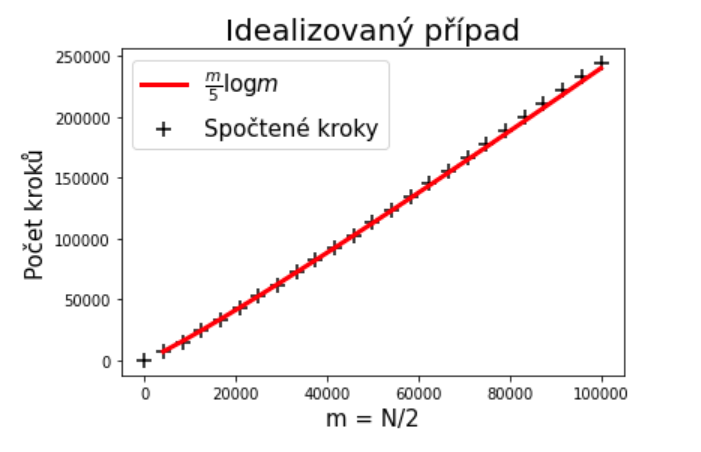
\includegraphics[height=5cm]{img/id2.png}
\end{figure}
\end{frame}



\end{document}